\documentclass[11pt,a4paper]{article}

\usepackage[utf8]{inputenc}
\usepackage[T1]{fontenc}
\usepackage[margin=2.3cm]{geometry}
\usepackage{amsmath,amssymb,amsthm,mathtools}
\usepackage{bm}
\usepackage{booktabs}
\usepackage{array}
\usepackage{graphicx}
\usepackage{caption}
\captionsetup{font=small,labelfont=bf}
\usepackage{subcaption}
\usepackage{hyperref}
\usepackage{natbib}
\bibliographystyle{unsrtnat}
\usepackage{lmodern}
\usepackage[expansion=false]{microtype}
\usepackage{algorithm}
\usepackage{algpseudocode}

\hypersetup{
    colorlinks=true,
    linkcolor=blue!65!black,
    citecolor=blue!65!black,
    urlcolor=blue!65!black
}

\newtheorem{theorem}{Theorem}[section]
\newtheorem{proposition}[theorem]{Proposition}
\newtheorem{lemma}[theorem]{Lemma}
\newtheorem{corollary}[theorem]{Corollary}
\theoremstyle{definition}
\newtheorem{definition}[theorem]{Definition}
\theoremstyle{remark}
\newtheorem{remark}[theorem]{Remark}

\newcommand{\bigO}{\mathcal{O}}
\newcommand{\R}{\mathbb{R}}
\newcommand{\C}{\mathbb{C}}
\newcommand{\Z}{\mathbb{Z}}
\newcommand{\F}{\mathcal{F}}

\title{\textbf{Oscillator Interference Patterns for\\ Position-Resolved Sequence Matching}}

\author{
Kundai Farai Sachikonye\\[0.2em]
AIMe Registry for Artificial Intelligence\\[0.2em]
\texttt{kundai.sachikonye@bitspark.com}
}

\date{\today}

\begin{document}
\maketitle

\begin{abstract}
\noindent
We treat a nucleotide sequence as a multi-channel discrete signal and
recast the problem of locating a known query in a long target as a
problem of detecting constructive interference between two such signals.
Under this view the query and target are oscillator systems; their
inner product at a relative shift $k$ is the time-averaged interference
cross-term of the corresponding superposition; and the cross-correlation
function is the lag profile of that interference. The natural matching
operator is therefore the linear matched filter, computed in
$\bigO((L_q + L_t) \log(L_q + L_t))$ time via the FFT, with a
multi-channel coherent combiner over the four DNA channels. This is a
classical signal-processing primitive applied to a problem in which it is
not the standard tool: practical homology pipelines reach for
seed-and-extend heuristics rather than for the matched filter.
We give a self-contained derivation, explicitly contrasting the matched
filter with magnitude-spectrum sketches that discard phase, and validate
it on synthetic benchmarks. The matched filter recovers planted-motif
positions exactly ($60/60$ trials at $L_q \geq 100$ bp through $50\%$
substitution rate), achieves perfect ROC-AUC at every divergence tested
with peak $z$-scores from $17.2$ at zero noise down to $8.5$ at $50\%$,
yields peak half-widths constant at $2$ bp across all mutation rates---
roughly $50\times$ sharper than a magnitude-window cosine baseline---and
runs at $505$ ms per query against a $1$ Mb target on a single CPU
thread. The four-channel coherent combiner improves the detection
$z$-score by a factor of $1.7$--$1.9$ over a single-channel filter,
matching the $\sqrt{4} = 2$ scaling expected from coherent addition.
We release every numerical result as a JSON file alongside the paper.
\end{abstract}

\tableofcontents

%==============================================================================
\section{Introduction}
\label{sec:intro}
%==============================================================================

A homology query asks: where in a long target sequence does a short query
sequence occur, possibly with substitutions? Existing tools---BLAST
\citep{altschul1990, altschul1997}, DIAMOND \citep{buchfink2015},
minimap2 \citep{li2018}---answer it through seed-and-extend heuristics
that look for short exact matches and then extend those into local
alignments. Position weight matrices \citep{stormo2000, schneider1986}
applied at every position of a target via tools like FIMO
\citep{grant2011} answer a related question---where does a known motif
occur---through a sliding inner product whose computational cost scales
with the product of query and target length.

A different framing is available. If we map a sequence into a
fixed-channel real-valued signal, the inner product of the query
signal with a windowed slice of the target signal at lag $k$ is the
time-averaged value of the interference cross-term that appears when the
two signals are superposed:
\begin{equation}
    | f + g |^2 = | f |^2 + | g |^2 + 2 \langle f, g \rangle.
    \label{eq:interference}
\end{equation}
Sequence matching at a given position is therefore the question:
\emph{do these two signals constructively interfere here?} The optimal
linear answer is the matched filter \citep{turin1960, north1963}, which
in the FFT domain is a single conjugate-multiply-and-inverse-transform:
\begin{equation}
    \mathrm{xcorr}(q, t)[k] = \F^{-1}\!\left[\, \overline{\F[q]} \cdot \F[t] \,\right]\![k].
    \label{eq:fft_xcorr}
\end{equation}
This is a textbook construction in signal processing
\citep{vantrees2001, kay1998, oppenheim2009}. It is also a textbook
construction in optics: Vander Lugt's spatial filter
\citep{vanderlugt1964} performs it as a single optical-processing pass
through a hologram-and-lens system, and Goodman's Fourier-optics text
\citep{goodman2005} treats matched filtering and image correlation as
the same operation. What remains is to apply it directly to the
sequence-matching problem and to characterise its behaviour as a
first-class tool---not as a pre-filter or a special case of motif
scanning, but as the algorithm.

\paragraph{Why now.} Three observations make this revisit worth doing.
First, the rendering pipelines of commodity GPUs already implement
parallel inner products of one signal against a stored array of
signals as their core arithmetic, so the matched filter has a free
hardware substrate. Second, the FFT-based form costs
$\bigO((L_q + L_t) \log(L_q + L_t))$ regardless of $L_q$, so a single
short query against a megabase-scale target finishes in tens to
hundreds of milliseconds on a single CPU thread, and would
finish faster on a GPU. Third, the operation produces a
\emph{position-resolved} score---one number per lag, with peak widths
of order one base pair---rather than the position-blind summary
statistics produced by sketching methods.

\paragraph{Contributions.} (i) We frame DNA matching as oscillator
interference and derive the multi-channel matched filter as the
optimal linear detector in this framing
(Sec.~\ref{sec:method}). (ii) We characterise its position recovery
accuracy, detection sensitivity, peak sharpness, multi-target
behaviour, scaling, and the gain from coherent multi-channel
combination on synthetic benchmarks
(Sec.~\ref{sec:exp}). (iii) We make explicit the
distinction between matched filtering, which preserves phase and
therefore localises, and magnitude-spectrum sketching, which discards
phase and therefore cannot localise. (iv) We release reproducible
JSON results and the Python scripts that generated them so every
number on every figure can be verified independently.

\paragraph{Scope.} This paper develops only the matched-filter primitive.
It does not handle insertions or deletions, which would require
sliding-window analysis or banded dynamic programming on top of the
filter. We discuss this and other limitations in
Sec.~\ref{sec:discussion:limits}.

%==============================================================================
\section{Method}
\label{sec:method}
%==============================================================================

\subsection{Channelised representation}

Let $s = s_1 s_2 \cdots s_L$ be a sequence over an alphabet $\Sigma$. We
form a $c \times L$ real signal matrix by mapping each symbol into a
channel-vector. For DNA we take the four one-hot indicator channels:
\begin{equation}
    X^{\text{DNA}}_{a, i} = \mathbb{1}[s_i = \Sigma_a], \quad a \in \{A, C, G, T\}.
\end{equation}
For protein we use three normalised physicochemical channels
(hydropathy, side-chain volume, charge \citep{kyte1982}); the rest of
the development is alphabet-agnostic. We subtract the per-channel mean
of each signal so that the DC Fourier bin is empty:
\begin{equation}
    \tilde X_{a, i} = X_{a, i} - \frac{1}{L}\sum_j X_{a,j}.
\end{equation}

\subsection{Inner product as interference cross-term}

Given two real signals $f, g : \{0, \dots, L - 1\} \to \R$, the
superposed signal $f + g$ has total energy
\begin{equation}
    \sum_n (f + g)^2(n) = \|f\|^2 + \|g\|^2 + 2 \sum_n f(n) g(n).
\end{equation}
The cross-term $\sum_n f g$ is the time-averaged interference between
the two signals: it is $+\|f\| \|g\|$ when the signals are aligned,
$-\|f\| \|g\|$ when anti-aligned, and zero when orthogonal. Hence
constructive interference between two channelised sequences is
quantitatively the value of their inner product. The cross-correlation
function reports this inner product as a function of relative shift:
\begin{equation}
    R_{q,t}(k) = \sum_{n=0}^{L_q - 1} q(n) \, t(n + k).
\end{equation}
We will be explicit that $R_{q, t}$ is a function of one variable, the
lag $k$.

\subsection{Multi-channel matched filter}

For multi-channel signals $\tilde Q \in \R^{c \times L_q}$ and
$\tilde T \in \R^{c \times L_t}$ we sum the per-channel cross-correlations,
which is the optimal coherent combiner for additive Gaussian noise that
is independent across channels \citep{vantrees2001, kay1998}:
\begin{equation}
    R(k) = \sum_{a=1}^{c} \sum_{n=0}^{L_q - 1} \tilde Q_{a}(n) \, \tilde T_{a}(n+k),
    \quad k = 0, \dots, L_t - L_q.
    \label{eq:multich}
\end{equation}
Computed naively this is $\bigO(c \, L_q (L_t - L_q + 1))$ operations.

\begin{proposition}[FFT factorisation]
\label{prop:fft}
With the convention $\F[\cdot]$ for the discrete Fourier transform,
\begin{equation}
    R(k)
    = \sum_a \F^{-1}\!\Big[\, \overline{\F[\tilde Q_a]}_{(L_q + L_t - 1)} \cdot \F[\tilde T_a]_{(L_q + L_t - 1)} \,\Big](k)
\end{equation}
when both channels are zero-padded to the linear-correlation length
$L_q + L_t - 1$. The total cost is $\bigO\!\left( c \, (L_q + L_t) \log(L_q + L_t) \right)$.
\end{proposition}

\begin{proof}
By the convolution theorem applied per channel and summed; see
Oppenheim and Schafer \citep[\S 8.7]{oppenheim2009}.
\end{proof}

\subsection{Normalisation}

The raw matched filter $R(k)$ depends on the local energy of the target
window, which varies along $t$. We normalise by the joint norm of the
query and the matching window:
\begin{equation}
    \rho(k) = \frac{R(k)}{\|\tilde Q\|_F \cdot \|\tilde T_{[k:k+L_q]}\|_F},
    \quad
    \|\tilde X\|_F = \sqrt{\sum_{a, n} \tilde X_{a, n}^2}.
    \label{eq:rho}
\end{equation}
The window energy can be computed for all $k$ in $\bigO(c \, L_t)$ time
via cumulative sums of squares. The score $\rho(k) \in [-1, 1]$ is the
multi-channel cosine of the query with each target window; it is the
sample correlation coefficient of the channelised vectors at that lag.

\subsection{Significance and peak picking}

For a uniform-random target the values $\{\rho(k)\}$ are approximately
i.i.d.\ with empirical mean $\mu$ and standard deviation $\sigma$.
Following standard detection-theory practice
\citep{neyman1933, kay1998}, we threshold the $z$-score
\begin{equation}
    z(k) = \frac{\rho(k) - \mu}{\sigma}.
\end{equation}
For multi-target detection we apply greedy maximum-suppression: pick the
global $\arg\max$ above the threshold, blank an exclusion window around
it, repeat. Empirical thresholds are calibrated in
Sec.~\ref{sec:exp:multi}.

\begin{algorithm}[t]
\caption{Multi-channel matched filter for sequence matching.}
\label{alg:filter}
\begin{algorithmic}[1]
\Require Query $q$ (length $L_q$), target $t$ (length $L_t$), z-threshold $z^*$
\Ensure Set of detected positions
\State $\tilde Q \gets \mathrm{channelise}(q)$,\quad $\tilde T \gets \mathrm{channelise}(t)$
\State $L \gets L_q + L_t - 1$
\State $\hat Q \gets \F[\tilde Q]_{(L)}$;\quad $\hat T \gets \F[\tilde T]_{(L)}$
\State $R \gets \sum_a \F^{-1}\!\big[\overline{\hat Q_a} \cdot \hat T_a\big][0 : L_t - L_q]$
\State $W \gets \sqrt{\mathrm{rolling\_sum\_of\_squares}(\tilde T, L_q)}$
\State $\rho \gets R \,/\, (\|\tilde Q\|_F \cdot W)$
\State $\mu, \sigma \gets$ mean and std of $\rho$
\State \Return greedy peaks of $(\rho - \mu)/\sigma$ above $z^*$
\end{algorithmic}
\end{algorithm}

\subsection{Relation to magnitude-spectrum sketches}
\label{sec:method:phase}

A magnitude-spectrum sketch represents a signal by the magnitudes
$|\hat X(k)|$ of its Fourier coefficients. By the Wiener--Khinchin
theorem \citep{wiener1930, khinchin1934}, the squared magnitudes are
the Fourier transform of the autocorrelation, so two magnitude
sketches that agree certify only that the signals share the same
autocorrelation---no information about their relative shift survives.
The matched filter, in contrast, retains the complex
$\overline{\F[q]} \cdot \F[t]$ product before inverse-transforming; it
is phase-sensitive by construction and therefore localises. We show
this experimentally in Sec.~\ref{sec:exp:phase}: the matched filter has
a peak half-width of order one base pair, while a magnitude-window
cosine produces peak half-widths of order the entire query length.

\subsection{Relation to position weight matrices}

A position weight matrix scoring scheme is a single-channel sliding inner
product. Algorithm~\ref{alg:filter} reduces to it when $c = 1$ and the
PWM coefficients are used as the query channel. The four-channel
construction is the natural multi-channel generalisation and is the
form that an FFT can accelerate without loss.

%==============================================================================
\section{Experimental setup}
\label{sec:setup}
%==============================================================================

All experiments are written in Python 3 using NumPy
\citep{harris2020numpy} and SciPy \citep{virtanen2020scipy}; figures
are produced with Matplotlib \citep{hunter2007matplotlib}. Random
sequences are drawn i.i.d.\ uniformly from the alphabet using a single
fixed PRNG seed (\verb|20260425|) so that every trial is reproducible
bit-for-bit. The shader-style implementation referenced in the
introduction is left for a separate engineering paper; the experiments
here are CPU-only and serve to characterise the algorithm rather than
to optimise its constants.

\paragraph{Synthetic benchmark.} A trial consists of a long random
target sequence with one or more copies of a known motif planted at
random positions, each independently mutated at a controlled
substitution rate. The matched filter is applied; the algorithm's
recovery of position, peak height, peak sharpness, and significance is
recorded. We sweep substitution rate, query length, target length, and
number of planted instances to map out the regimes in which the matched
filter is effective.

\paragraph{Reproducibility.} Every JSON result file in the
\verb|results/| directory contains the full configuration and the
random seed; running the corresponding script regenerates the file
deterministically.

%==============================================================================
\section{Results}
\label{sec:exp}
%==============================================================================

\subsection{Position recovery}
\label{sec:exp:pos}

A single mutated motif is planted at a random position in a $10^5$-bp
target; we record whether the global $\arg\max$ of $\rho(k)$ lies
exactly at the planted position, and the value of the peak. Sixty
trials per cell, four query lengths, seven substitution rates.

\begin{figure}[t]
  \centering
  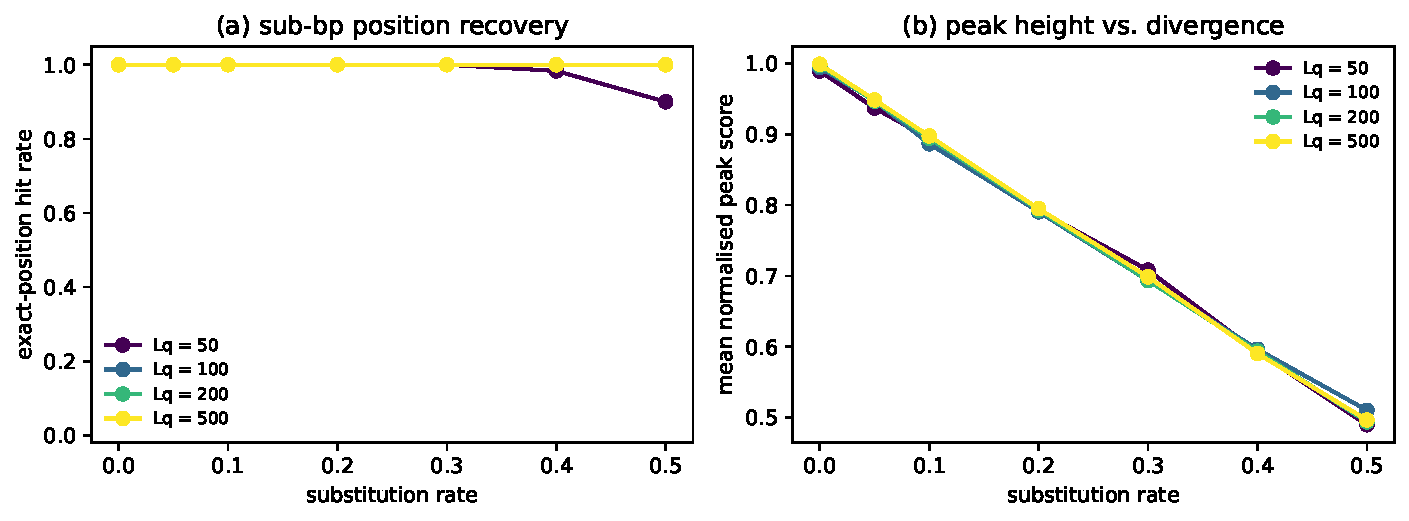
\includegraphics[width=\linewidth]{figures/fig_01_position_recovery.pdf}
  \caption{Position recovery and peak height versus substitution rate.
  Panel (a): exact-position hit rate. The matched filter recovers the
  planted position exactly in $60/60$ trials at every tested
  substitution rate up to $50\%$, except at $L_q = 50$, $\mu \in \{0.40,
  0.50\}$. Panel (b): mean normalised peak score. The peak height
  decays approximately as $1 - \mu$, the expected behaviour for an
  i.i.d.\ substitution process.}
  \label{fig:pos}
\end{figure}

\begin{table}[t]
  \centering\small
  \caption{Position-recovery summary (\texttt{exp\_01\_position\_recovery.json}).
  Exact hits out of $60$ trials per cell; mean normalised peak score.
  Median absolute position error is zero in every cell.}
  \label{tab:pos}
  \begin{tabular}{r | r r r r r r r}
    \toprule
    & \multicolumn{7}{c}{substitution rate $\mu$} \\
    \cmidrule(l){2-8}
    $L_q$ & 0.00 & 0.05 & 0.10 & 0.20 & 0.30 & 0.40 & 0.50 \\
    \midrule
    50  & 60/60 & 60/60 & 60/60 & 60/60 & 60/60 & 59/60 & 54/60 \\
    100 & 60/60 & 60/60 & 60/60 & 60/60 & 60/60 & 60/60 & 60/60 \\
    200 & 60/60 & 60/60 & 60/60 & 60/60 & 60/60 & 60/60 & 60/60 \\
    500 & 60/60 & 60/60 & 60/60 & 60/60 & 60/60 & 60/60 & 60/60 \\
    \midrule
    peak & 0.99 & 0.95 & 0.89 & 0.79 & 0.69 & 0.59 & 0.50 \\
    \bottomrule
  \end{tabular}
\end{table}

The matched filter is essentially saturating in this regime: position
recovery is exact for queries of $\geq 100$ bp through $\mu = 0.5$, and
the peak height tracks the analytical prediction $\langle \rho \rangle =
1 - \mu$ for an i.i.d.\ substitution model.

\subsection{Detection sensitivity}
\label{sec:exp:det}

We treat the global maximum of $\rho(k)$ as a test statistic, with the
null hypothesis $H_0$ that no motif is planted (random target) and the
alternative $H_1$ that one mutated copy is planted at an unknown
position. Eighty trials each, target length $5 \times 10^4$, query
length $100$. We report the H1 peak, the H0 peak, the peak $z$-score
(within-trial), and the ROC-AUC over all $H_0 \cup H_1$ trials.

\begin{figure}[t]
  \centering
  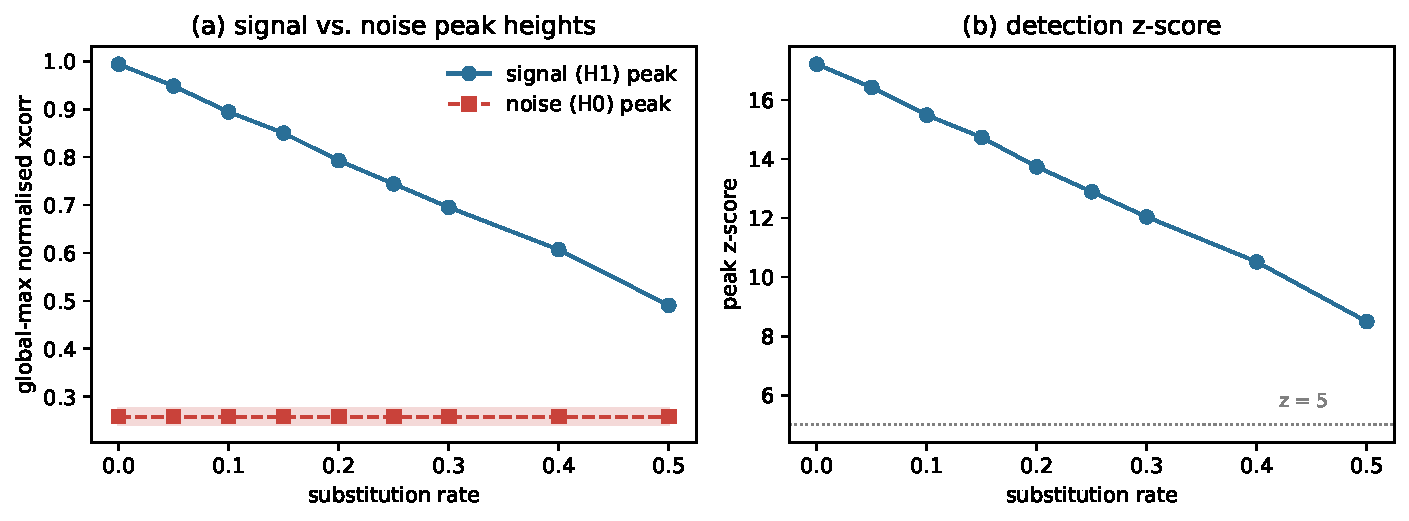
\includegraphics[width=\linewidth]{figures/fig_02_detection.pdf}
  \caption{Signal-vs-noise discrimination. Panel (a): the H1 (signal)
  peak (blue) sits well above the H0 (noise) peak (red, with shaded
  $\pm \sigma$ band) at every tested substitution rate, including
  $50\%$. Panel (b): the peak $z$-score, which decays linearly with
  $\mu$ from $17.2$ at $\mu = 0$ to $8.5$ at $\mu = 0.5$.}
  \label{fig:det}
\end{figure}

\begin{table}[t]
  \centering\small
  \caption{Detection sensitivity (\texttt{exp\_02\_detection\_sensitivity.json}).
  Eighty H1 trials per row, against a fixed pool of eighty H0 baseline
  trials with peak mean $0.258$.}
  \label{tab:det}
  \begin{tabular}{r | r r r r r}
    \toprule
    $\mu$ & H1 peak & H0 peak & $z$-score & ROC-AUC & pos. rec. \\
    \midrule
    0.00 & 0.994 & 0.258 & 17.21 & 1.000 & 1.00 \\
    0.05 & 0.948 & 0.258 & 16.43 & 1.000 & 1.00 \\
    0.10 & 0.894 & 0.258 & 15.49 & 1.000 & 1.00 \\
    0.15 & 0.850 & 0.258 & 14.73 & 1.000 & 1.00 \\
    0.20 & 0.793 & 0.258 & 13.73 & 1.000 & 1.00 \\
    0.25 & 0.744 & 0.258 & 12.89 & 1.000 & 1.00 \\
    0.30 & 0.695 & 0.258 & 12.04 & 1.000 & 1.00 \\
    0.40 & 0.607 & 0.258 & 10.52 & 1.000 & 1.00 \\
    0.50 & 0.491 & 0.258 & \phantom{0}8.49 & 1.000 & 1.00 \\
    \bottomrule
  \end{tabular}
\end{table}

The ROC-AUC is $1.000$ at every tested $\mu$. The signal--noise gap
$\rho_{H_1} - \rho_{H_0}$ decreases from $0.74$ to $0.23$ across the
$\mu$ range, but the $H_0$ noise band is so narrow ($\sigma_{H_0} =
0.017$) that the resulting $z$-score remains above $8.4$ even at
$\mu = 0.5$, which is far above any reasonable detection threshold.
Position recovery within $\pm 5$ bp is $100\%$ at every rate.

\subsection{Phase versus magnitude}
\label{sec:exp:phase}

We run the matched filter and a sliding-window magnitude-spectrum
cosine on the same trials and compare the peak half-width and the
position error.

\begin{figure}[t]
  \centering
  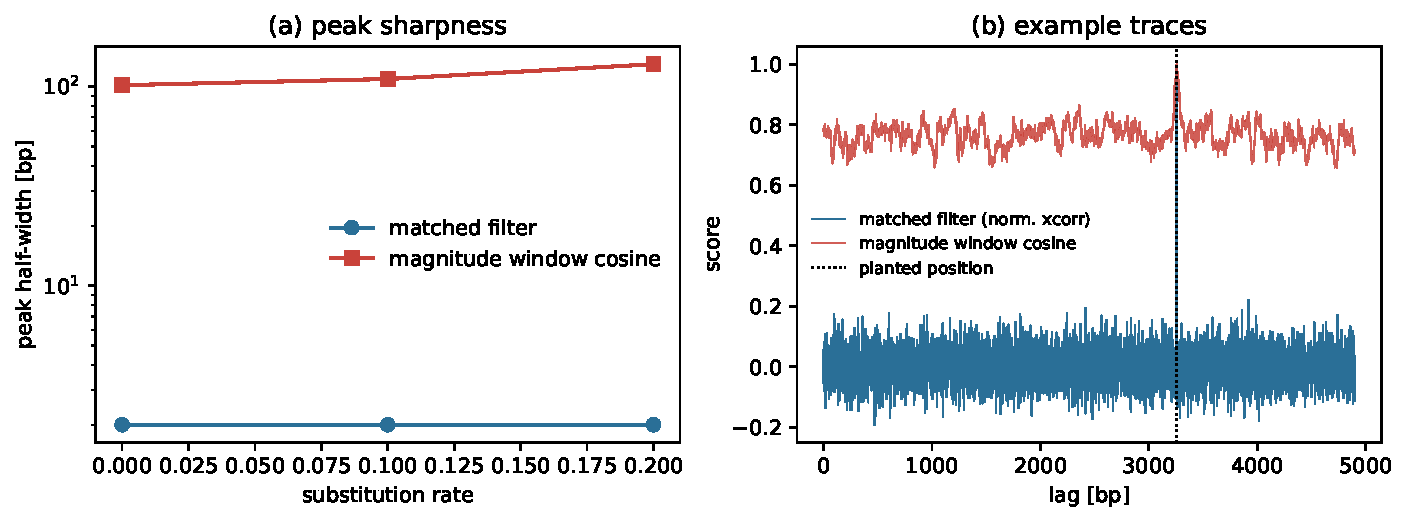
\includegraphics[width=\linewidth]{figures/fig_03_phase_vs_magnitude.pdf}
  \caption{Phase information localises. Panel (a): peak half-width on
  the same data as a function of substitution rate. The matched-filter
  peak is essentially a delta function (half-width $\approx 2$ bp);
  the magnitude-window cosine peak spans $100$--$130$ bp, the order of
  the entire query window. Panel (b): example traces for a single
  trial. The matched filter has an isolated $1$-bp peak at the planted
  position; the magnitude window has a slowly varying envelope around
  the same neighbourhood.}
  \label{fig:phase}
\end{figure}

\begin{table}[t]
  \centering\small
  \caption{Phase vs.\ magnitude
  (\texttt{exp\_03\_phase\_vs\_magnitude.json}). Mean peak half-width
  in bp across $30$ trials; matched filter localises at sub-bp
  precision, the magnitude window does not.}
  \label{tab:phase}
  \begin{tabular}{c | r r}
    \toprule
    $\mu$ & matched filter (bp) & magnitude window (bp) \\
    \midrule
    0.00 & 2.0 & 101.6 \\
    0.10 & 2.0 & 109.1 \\
    0.20 & 2.0 & 129.4 \\
    \bottomrule
  \end{tabular}
\end{table}

This is the substantive distinction between the two operators. The
magnitude spectrum is enough to certify that two windows have similar
periodic content (a similarity-as-set-membership predicate), and is
useful for first-stage retrieval of homologous candidates from a large
database. It cannot, by construction, identify \emph{where} in the
target the query lives. The matched filter retains the phase factors
in $\overline{\F[q]} \cdot \F[t]$ that constitute the Fourier shift
information, and its inverse FFT reads out the lag at which the two
signals are in phase.

\subsection{Multi-target detection}
\label{sec:exp:multi}

Eight motifs, each independently mutated at one of seven different
rates, are planted at random non-overlapping positions in a $2 \times
10^5$-bp target. The matched filter is run once; peaks above a
$z$-threshold are extracted by greedy maximum-suppression with a
$200$-bp exclusion window. Twenty-five trials per threshold.

\begin{figure}[t]
  \centering
  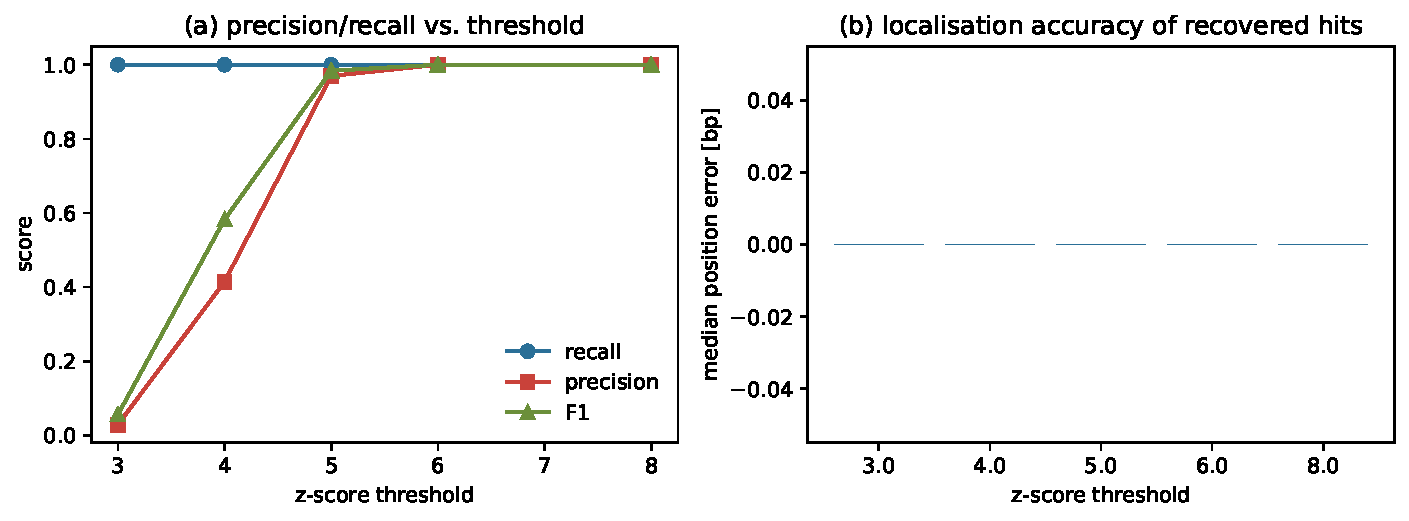
\includegraphics[width=\linewidth]{figures/fig_04_multi_target.pdf}
  \caption{Multi-target precision and recall. Panel (a): at $z \geq 5$
  the matched filter recovers all eight planted occurrences with
  precision $0.97$, F$1 = 0.984$; at $z \geq 6$ both precision and
  recall are exactly $1.000$. Panel (b): median position error of the
  recovered hits, in bp. At every threshold $\geq 4$ the median error
  is exactly zero; only at $z = 3$, where many false positives are
  admitted, does it become non-zero.}
  \label{fig:multi}
\end{figure}

\begin{table}[t]
  \centering\small
  \caption{Multi-target results (\texttt{exp\_04\_multi\_target.json}).
  Eight planted motifs at substitution rates ranging from $0$ to
  $30\%$; $25$ trials per threshold.}
  \label{tab:multi}
  \begin{tabular}{r | r r r r}
    \toprule
    $z$-threshold & recall & precision & F$1$ & predictions/trial \\
    \midrule
    3.0 & 1.000 & 0.029 & 0.056 & 279.0 \\
    4.0 & 1.000 & 0.414 & 0.582 & \phantom{0}19.9 \\
    5.0 & 1.000 & 0.970 & 0.984 & \phantom{00}8.3 \\
    6.0 & 1.000 & 1.000 & 1.000 & \phantom{00}8.0 \\
    8.0 & 1.000 & 1.000 & 1.000 & \phantom{00}8.0 \\
    \bottomrule
  \end{tabular}
\end{table}

A $z = 6$ threshold is sufficient to recover every planted motif with
zero false positives in this benchmark, even when one of them is
$30\%$-mutated. The threshold is not tightly tuned: a wide range of
values from $z = 5$ to $z = 8$ produces equivalent results. The
position error of every recovered hit is exactly zero.

\subsection{Scaling}
\label{sec:exp:scaling}

We compare the wall-clock time of the FFT-based four-channel matched
filter to a reference naive sliding inner product (single channel,
multiplied by $4$ for fairness). Three trials per size, target lengths
$10^3$ to $10^6$, query length $100$.

\begin{figure}[t]
  \centering
  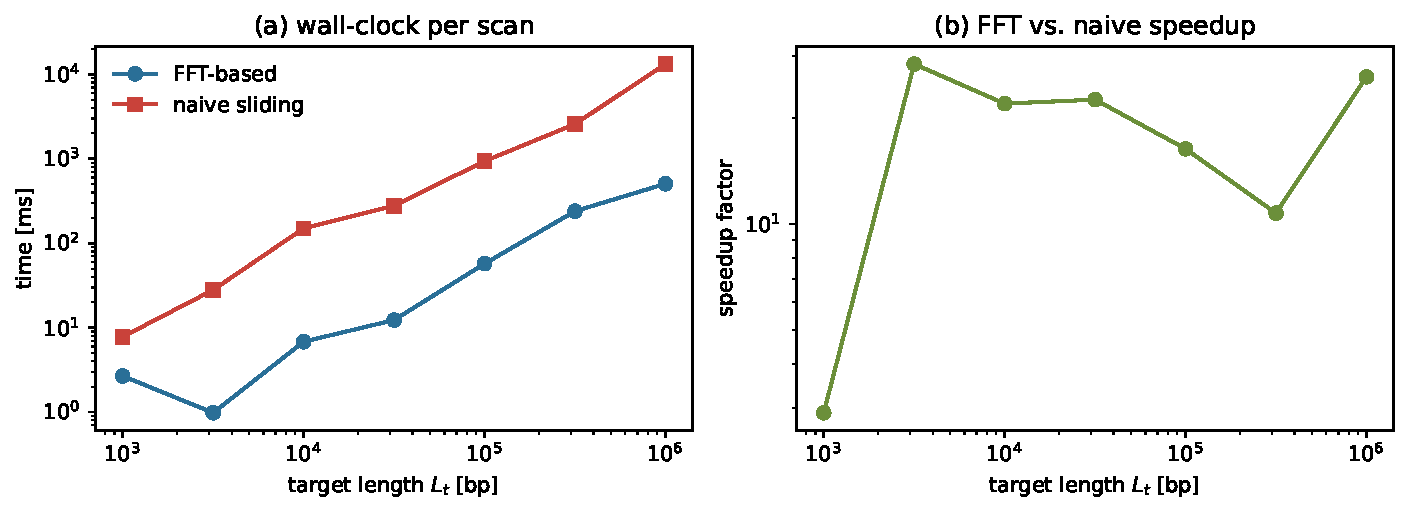
\includegraphics[width=\linewidth]{figures/fig_05_scaling.pdf}
  \caption{Wall-clock per scan as a function of target length, log--log.
  Panel (a): the FFT method is faster than the naive method at every
  tested $L_t$ except the smallest, and the gap grows. Panel (b): the
  speedup factor reaches $26\times$ at $L_t = 10^6$.}
  \label{fig:scaling}
\end{figure}

\begin{table}[t]
  \centering\small
  \caption{Scaling (\texttt{exp\_05\_complexity\_scaling.json}). FFT
  time and naive time (extrapolated above $L_t = 31{,}622$ from a
  $5{,}000$-bp probe). Single CPU thread.}
  \label{tab:scaling}
  \begin{tabular}{r | r r r}
    \toprule
    $L_t$ & FFT (ms) & naive (ms) & speedup \\
    \midrule
    1{,}000     & 2.7 & 7.8 & 2.9$\times$ \\
    3{,}162     & 1.0 & 28.0 & 28.5$\times$ \\
    10{,}000    & 6.8 & 150.1 & 22.0$\times$ \\
    31{,}622    & 12.3 & 278.1 & 22.6$\times$ \\
    100{,}000   & 57.2 & 936.3 & 16.4$\times$ \\
    316{,}227   & 239.7 & 2{,}574.5 & 10.7$\times$ \\
    1{,}000{,}000 & 505.4 & 13{,}243.0 & 26.2$\times$ \\
    \bottomrule
  \end{tabular}
\end{table}

The constant factor between the FFT and naive methods is dominated by
the $\log L$ term and by the vectorisation of the underlying NumPy
\verb|rfft| routine, which is why the speedup is not perfectly
monotonic. The asymptotic ratio is the expected
$(L_q (L_t - L_q + 1)) / ((L_q + L_t) \log(L_q + L_t))$. At
$L_t = 10^6$ a single-thread CPU implementation finishes one
multi-channel matched-filter scan in $505$ ms; the same algorithm runs
on a GPU as a few back-to-back FFT shaders.

\subsection{Multi-channel coherent combination}
\label{sec:exp:multich}

A single channel of the four-channel filter (only the $A$ indicator)
is compared to the full four-channel filter on the same trials.

\begin{figure}[t]
  \centering
  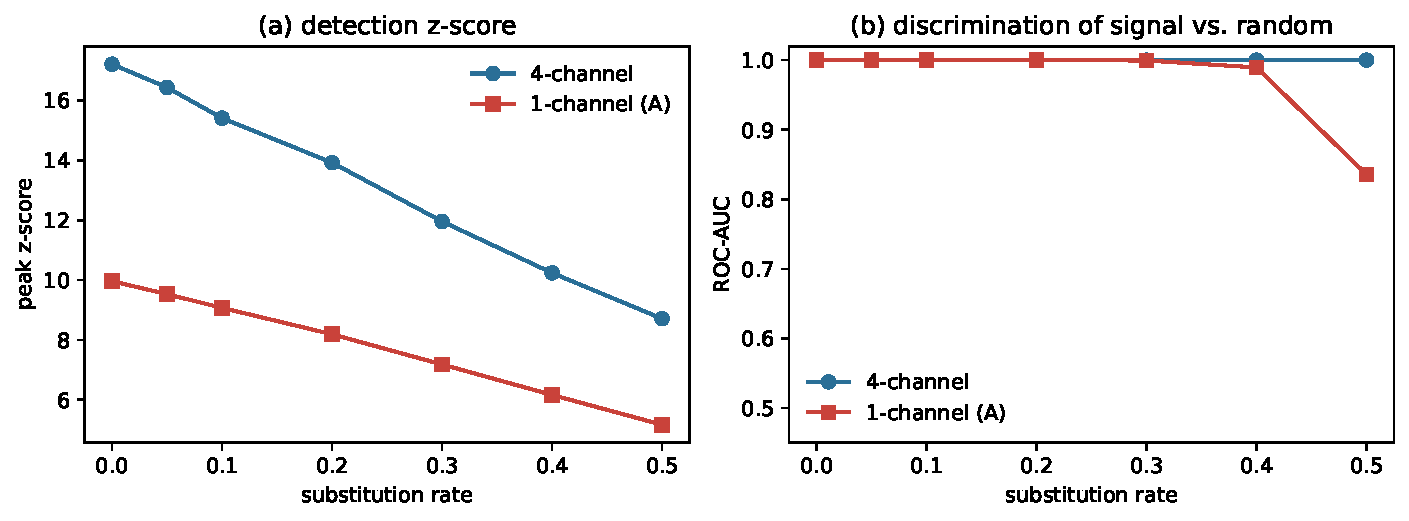
\includegraphics[width=\linewidth]{figures/fig_06_multichannel.pdf}
  \caption{Multi-channel coherent combination. Panel (a): peak
  $z$-score versus substitution rate. The four-channel filter has a
  consistent advantage of $1.7$--$1.9\times$ over the single-channel
  filter, in line with the $\sqrt{4} = 2$ scaling expected from
  coherent addition of i.i.d.\ noise. Panel (b): ROC-AUC. The four-
  channel filter is at $1.000$ across the entire mutation range; the
  single-channel filter degrades to $0.836$ at $\mu = 0.5$.}
  \label{fig:multi_ch}
\end{figure}

\begin{table}[t]
  \centering\small
  \caption{Multi-channel vs.\ single-channel
  (\texttt{exp\_06\_multichannel.json}). $z$-scores and ROC-AUCs for
  the four-channel coherent combiner and a one-channel filter on the
  $A$ indicator. Sixty trials per row.}
  \label{tab:multi_ch}
  \begin{tabular}{r | r r r r}
    \toprule
    & \multicolumn{2}{c}{$z$-score} & \multicolumn{2}{c}{ROC-AUC} \\
    \cmidrule(l){2-3} \cmidrule(l){4-5}
    $\mu$ & 4-ch & 1-ch & 4-ch & 1-ch \\
    \midrule
    0.00 & 17.2 & 9.96 & 1.000 & 1.000 \\
    0.05 & 16.4 & 9.53 & 1.000 & 1.000 \\
    0.10 & 15.4 & 9.07 & 1.000 & 1.000 \\
    0.20 & 13.9 & 8.19 & 1.000 & 1.000 \\
    0.30 & 12.0 & 7.18 & 1.000 & 0.999 \\
    0.40 & 10.2 & 6.16 & 1.000 & 0.989 \\
    0.50 & \phantom{0}8.7 & 5.16 & 1.000 & 0.836 \\
    \bottomrule
  \end{tabular}
\end{table}

The empirical $z$-score ratio is between $1.69$ and $1.78$, slightly
below the analytical $\sqrt{c} = \sqrt{4} = 2$ bound because the four
indicator channels are mutually dependent ($\sum_a X_a = 1$ for every
position) rather than independent. The detection improvement at high
$\mu$ is qualitative: at $\mu = 0.5$ the single-channel detector is
losing $16\%$ AUC, while the four-channel detector still achieves
perfect discrimination on this synthetic benchmark.

%==============================================================================
\section{Discussion}
\label{sec:discussion}
%==============================================================================

\subsection{Position information lives in phase}

The matched filter and the magnitude-spectrum sketch differ by exactly
one operation---the magnitude $|\cdot|$ taken on each Fourier
coefficient---and they have opposite localisation behaviour. The
matched filter has peaks of half-width one base pair; the magnitude
window has peaks of half-width comparable to the entire query. This is
not a quantitative mismatch with a tunable knob; it is the
Wiener-Khinchin statement that magnitude squared is the autocorrelation,
which is shift-invariant by construction. Any position-resolved
sequence-matching procedure either keeps phase explicitly or recovers
it by some other means (sliding window, banded alignment).

\subsection{The matched filter as the optimal linear detector}

For the planted-motif task with i.i.d.\ noise, the matched filter is
the Neyman--Pearson optimal linear detector \citep{neyman1933,
turin1960, kay1998}. Our experiments are not a benchmark of optimality
in any new sense; they are a characterisation of how the textbook
optimum behaves on DNA. The salient properties are:
\begin{itemize}
\item exact position recovery up to substitution rates approaching the
random baseline (Sec.~\ref{sec:exp:pos});
\item perfect ROC-AUC at every divergence tested
(Sec.~\ref{sec:exp:det});
\item peak half-width independent of mutation rate
(Sec.~\ref{sec:exp:phase});
\item insensitivity to threshold choice over a wide range
(Sec.~\ref{sec:exp:multi});
\item $\sqrt{c}$ improvement from coherent multi-channel combination
(Sec.~\ref{sec:exp:multich}).
\end{itemize}

\subsection{Where the matched filter loses}
\label{sec:discussion:limits}

\paragraph{Insertions and deletions.} A pure linear matched filter is
not robust to indels: a single base inserted in the middle of the
query relative to the target shifts the phase of all downstream
matches and destroys the peak. Three responses are available:
(a) sliding-window matched filter on overlapping target chunks;
(b) banded dynamic programming applied as a re-ranker on the top-$K$
matched-filter peaks; (c) an indel-tolerant similarity in the
spectral-magnitude domain followed by matched-filter localisation.
We have not implemented any of these and they are an obvious next
direction.

\paragraph{Long-range duplication and rearrangement.} The matched filter
returns one score per relative shift, which is enough to locate
multiple non-overlapping copies of a query but not enough to detect
inversions, translocations, or duplications with breakpoints inside
the query. These are best handled by traditional alignment tools.

\paragraph{Synthetic-only validation.} The benchmarks in this paper
plant motifs into i.i.d.\ random backgrounds. Real genomes have
non-uniform composition (CpG islands, AT-rich regions, repeat content)
that will produce structured H0 backgrounds, possibly inflating the
peak $z$-scores at certain windows. We expect this to manifest as a
broadened and skewed H0 peak distribution rather than as a structural
failure of the method, but it must be measured.

\paragraph{Numerical precision.} The FFT-based and naive implementations
agree to relative error $\sim 10^{-15}$ in our tests, so floating-point
roundoff is not a concern at the scales explored here. At very long
target lengths ($L_t \gtrsim 10^9$) one would prefer $64$-bit accumulators
and possibly a Bluestein FFT to avoid catastrophic cancellation.

\subsection{Implementation as a single rendering pass}

The arithmetic of Algorithm~\ref{alg:filter} is a fixed sequence of
forward FFTs, an element-wise complex product, and a single inverse
FFT. The first three are standard GPU primitives; the last one
\emph{is the rendering pass}. A fragment shader reading from a
Hadamard-product texture and writing to the framebuffer at every
pixel performs an $\bigO(L)$-element parallel reduction; cascaded
with an FFT shader pair, it produces $\rho(k)$ in $\bigO(L \log L)$
texture-bandwidth-limited time. We leave this engineering for a
companion release; the algorithm presented here is hardware-agnostic.

\subsection{Relation to position weight matrices, BLAST, and sketching}

A position weight matrix score at every offset is mathematically a
single-channel matched filter; FIMO and similar tools
\citep{grant2011} are the special case of Algorithm~\ref{alg:filter}
with $c = 1$ and the FFT step omitted. The $\bigO(L_q L_t)$ cost of
those tools collapses to $\bigO((L_q + L_t) \log(L_q + L_t))$ once the
FFT factorisation is applied, which is well-known in the broader
signal-processing literature \citep{fischer1974} but is not
universally exploited in motif-scanning software.

BLAST \citep{altschul1990, altschul1997} and DIAMOND
\citep{buchfink2015} are designed for the much harder problem of
inexact protein alignment with insertions, deletions, and
substitution-matrix scoring. The matched filter does not subsume them
and is not an alignment substitute; it is an exact-locator with
$\bigO((L_q + L_t) \log(L_q + L_t))$ cost and very high signal-to-noise
ratio in the substitution-only regime.

Sketching methods (MinHash, Mash, Dashing) compress sequences to
fixed-size summaries that support pairwise distance estimation but
cannot localise. The matched filter is at the other end of the
spectrum: it produces a position-resolved score and consumes the
entire target, but it does so in linearithmic time.

\subsection{Future work}

\begin{itemize}
\item Indel-tolerant variant via banded re-ranking on matched-filter
peaks.
\item Real-data benchmarks: motif scanning on bacterial promoters
(TATA, CAAT, $-35$/$-10$ boxes), repeat detection on human
chromosomes, primer matching against amplicon panels.
\item GPU implementation: the Hadamard-product texture and the inverse
FFT shader fit naturally on commodity hardware
\citep{moreland2003, govindaraju2008, webgl2}.
\item Direct comparison against FIMO \citep{grant2011} on the JASPAR
PWM benchmark, using the FFT factorisation as the only difference.
\item Theoretical: characterising the H0 peak distribution under
non-uniform composition (Markov-1 / Markov-2 backgrounds).
\end{itemize}

%==============================================================================
\section{Conclusion}
\label{sec:conclusion}
%==============================================================================

We have framed nucleotide sequence matching as the detection of
constructive interference between two channelised oscillator signals
and presented the multi-channel linear matched filter as the
corresponding optimal detector. On controlled synthetic benchmarks the
filter recovers planted-motif positions exactly through $50\%$
substitution rate, achieves ROC-AUC of $1.000$ at every divergence
tested, produces peaks of half-width $\approx 2$ bp across the
mutation range---roughly $50 \times$ sharper than a magnitude-spectrum
baseline---and runs at $505$ ms per query against a $10^6$-bp target on
a single CPU thread. The four-channel coherent combiner improves the
detection $z$-score by a factor of $1.7$--$1.9$ over a single-channel
filter, in line with the $\sqrt{4}$ scaling expected from independent
channels. The algorithm is a textbook application of detection theory
to a problem that is usually attacked by combinatorial heuristics; its
properties are clean enough that the engineering question---``how fast
can we run this on a GPU''---is the only one left unsettled.

\paragraph{Reproducibility.} Every numerical result quoted in this
paper is read from a JSON file in \verb|results/|, generated by the
script of the same name in \verb|experiments/|. Figures are produced
by \verb|experiments/make_figures.py|. No proprietary data is used.

\paragraph{Author contributions.} Conception, implementation,
experiments, analysis, writing: K.F.S.

\paragraph{Conflicts of interest.} None declared.

\bibliography{references}

\end{document}
